\chapter{Plotting}
\index{plotting}
\label{c:plotting}

\begin{figure}[b]
  \centering
  \includegraphics[width=4.5in]{plot-typical.pdf}
  \caption[An example of a plot display.]
{An example of a plot display. In this example there are three graphs: A graph displaying the beta
function, a graph displaying the orbit, and a graph displaying the ``lattice layout'' which shows
the longitudinal positions of lattice elements.}
  \label{f:plot.typ}
\end{figure}

\tao has a graphical display window within which such things as lattice functions, machine layout,
beam positions, etc., can be plotted. An example is shown in \fig{f:plot.typ} where there are plots
of the beta function and orbit along with a ``lattice layout which shows the longitudinal positions
of lattice elements. 

\tao organizes the display window using a number of concepts which are explained in the 
sections below
\begin{example}
  plot_page     ! The display window containing the graphics (\sref{s:plot.page.def}).
  regions       ! A set of rectangles on the plot_page that plots can be put in (\sref{s:region.def}).
  plot          ! A collection of graphs (\sref{s:plot.def}).
  box           ! Rectangular area within a plot that a graph is placed in (\sref{s:box.def}).
  graph         ! A diagram of some sort (\sref{s:graph.def}).
  curve         ! Data displayed within a \vn{graph} (\sref{s:curve.def}).
\end{example}

Underlying all this is the \vn{quick_plot} software toolkit (\sref{s:quick.plot}) which was developed
for \bmad and \tao for graphics plotting.

%-----------------------

\begin{figure}[bt]
  \centering
  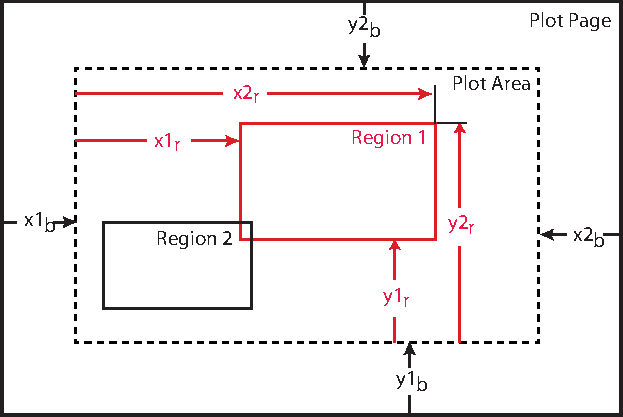
\includegraphics{plot-page.pdf}
  \caption[The plot window.]{The \vn{plot page} is the entire display window area. The \vn{plot area} 
is the region within the boarders of the \vn{plot page} within which ``\vn{regions}'' are
placed. The location of a \vn{region} is defined by four offsets with respect to the \vn{plot
area}. Regions may overlap.}
  \label{f:plot.page}
\end{figure}

%-----------------------------------------------------------------
\section{Plot Page}
\label{s:plot.page.def}

The \vn{plot page}, sometimes called the \vn{plot window}, refers to the window or the corresponding
printed graphics page where graphics are displayed. A \vn{plot page} is shown schematically in
\fig{f:plot.page}. Parameters associated with the \vn{plot page} are discussed in
\sref{s:plot.page}.  These parameters may be set in an initialization file or may be set on the \tao
command line using the \vn{set plot_page} (\sref{s:set.plot.page}) command. Examples:
\begin{example}
  set plot_page text_height = 11  ! 11 point font size
  set plot_page border%x1 = 0.2   ! Set left page border to 20% of width.
\end{example}

The size of the \vn{plot page} is set by the \vn{plot_page%size} parameter which is an array of two
numbers which set the width and height. The \vn{plot page} size can also be set when invoking \tao
using the \vn{-geometry} option (\sref{s:command.line})
\begin{example}
  > tao -lattice lat.bmad -geometry 300x500
\end{example}
This starts \tao with the \vn{plot page} size set to 300 points wide by 500 points high. It is also
sometimes convenient to start \tao without the plotting window. In this case, the \vn{-noplot} option
can be used on the startup command line. In a \tao initialization file, display of the plot window can be set
using the \vn{global%plot_on} parameter set in the \vn{tao_params} namelist (\sref{s:globals}).

In some cases, the screen resolution reported to \tao can be off. This has happened with some high
resolution displays where the reported resolution is 96 dpi when in fact the actual resolution is
much larger. In such a case, the size of the plot window created by \tao will be off. This can be
corrected by setting \vn{plot_page%size} appropriately but this in turn can create font size
problems. To avoid this problem, the environmental variable \vn{ACC_DPI_RESOLUTION} can be set to
the correct resolution before running \tao. The shell command line would be something like
\begin{example}
  > export ACC_DPI_RESOLUTION=168
\end{example}

The \vn{plot page} has a border within which \vn{regions} (\sref{s:region.def}) are defined. The area withing
the plot page border is called the \vn{plot area}

The \vn{show plot -page} (\sref{s:show.plot}) command may be used to view the page parameters.

%-----------------------------------------------------------------
\section{Region}
\label{s:region.def}

The \vn{plot area} is the area within the border of the \vn{plot page} as shown in
\fig{f:plot.page}.  In this \vn{plot area}, ``\vn{regions}'' can be defined which are invisible
rectangles where a \vn{plot} (\sref{s:plot.def}) can be placed. This is shown schematically in
\fig{f:plot.page}. Each region has a name and four numbers which specifies the location of the
region within the plot area. Regions may be defined by the user. In addition, for convenience, \tao
will define a number of regions. \tao defined regions will either begin with the letter ``\vn{r}''
or begin with the string ``\vn{layout}'' or the string ``\vn{scratch}''. Regions may overlap. How to
define regions is explained in \sref{s:plot.page}. The \vn{show plot} command will show the region
list. Example:
\begin{example}
  Tao> show plot

Plot Region         <-->  Plot                 x1    x2    y1    y2     Visible
-----------               -----------------------------------------------------
layout              <-->  lat_layout          0.00  1.00  0.00  0.15         T
r11                 <-->                      0.00  1.00  0.15  1.00
r12                 <-->                      0.00  1.00  0.58  1.00
r22                 <-->                      0.00  1.00  0.15  0.58
r13                 <-->  beta                0.00  1.00  0.72  1.00         T
r23                 <-->  dispersion          0.00  1.00  0.43  0.72         T
r33                 <-->  orbit               0.00  1.00  0.15  0.43         T
r14                 <-->                      0.00  1.00  0.79  1.00
\end{example}
The \vn{Plot} column shows what \vn{plot} (if any) is associated with the region
(\sref{s:plot.def}). The next four columns show the values of \vn{x1}, \vn{x2}, \vn{y1}, and \vn{y2}
set for the region. As shown in \Sref{s:plot.page}, \vn{x1} and \vn{x2} are the offsets from the
left \vn{plot area} edge to the left and right edges of the region. Similarly, \vn{y1} and \vn{y2}
are the offsets from the bottom edge of the \vn{plot area} to the bottom and top edges of the
region. \vn{x1} and \vn{x2} are normalized by the \vn{plot area} width and \vn{y1} and \vn{y2} are
normalized by the \vn{plot area} height so all four numbers should be in the range $[0, 1]$.  Using
the above example, the \vn{r23} region spans the full width of the \vn{plot area} (since \vn{x1} = 0
and \vn{x2} = 1), and occupies approximately the middle third vertically of the \vn{plot area}
(since \vn{y1} = 0.43 and \vn{y2} = 0.72).

The last column in the above shows if the \vn{plot} associated with the \vn{region} is
visible. Normally everything is visible. Invisibility is used in some special cases. For example,
when using a Graphical User Interface (GUI).

The \vn{set region} command can be used to set region parameters. Example:
\begin{example}
  set region r13 y1 = 0.8  ! Sets lower edge vertical position
\end{example}

%-----------------------------------------------------------------
\section{Plot}
\label{s:plot.def}

A \vn{plot} is essentially a collection of \vn{graphs}. This is shown schematically in
\fig{f:plot.plot} which shows a plot with two graph side by side.

Plots are divided into two groups. A \vn{template} plot defines how a \vn{displayed} plot is to be
constructed. That is, a \vn{template} plot defines what the associated \vn{graphs} are, defines
graph placement within the plot, etc. When a \vn{template} plot is \vn{placed} in a \vn{region},
either by using the \vn{place} command (\sref{s:place}) or by placement defined in an initialization
file (\sref{s:plot.page}), the information of the \vn{template} is copied in order to construct a
\vn{displayed} plot. A given \vn{template} plot may be placed in multiple \vn{regions} to give
multiple \vn{displayed} plots and then, using \vn{set} commands, the data displayed in each of these
plots may be manipulated separately. For example, one displayed orbit plot could show the orbit of
the \vn{model} lattice while another orbit plot could show the orbit difference between the
\vn{model} and \vn{design} lattices. When a \vn{plot} is displayed in a given \vn{region},
everything drawn is scaled to the region size.

Use the \vn{show plot} to see what displayed plots are associated with what regions. Use the
\vn{show plot -templates} command to see a list of \vn{template} plots. \tao defines a number of
default \vn{template} plots. Section~\sref{s:template} discusses how to define custom template
plots in an initialization file. Use the \vn{set plot} command (\sref{s:set.plot}) to modify either
\vn{template} or \vn{displayed} plots.

All plots have a name. A \vn{displayed} plot will inherit the same name of the \vn{template} plot it
came from. If a given \vn{template} plot is used to create multiple \vn{displayed} plots. All of
these plots will have the same name. A \vn{displayed} plot can also be referred to by using the
associated \vn{region} name. This can be used to remove ambiguity if there are multiple
\vn{displayed} plots of the same name. Additionally, a \vn{template} plot can unambiguously be
referred to by adding the prefix ``\vn{T::}'' to the plot name. Examples:
\begin{example}
  show plot           ! Show plots associated with regions
  show plot -template ! Show template plots
  place r13 orbit     ! Put orbit template into r13 region
\end{example}

Some commands, for example, the \vn{scale} command by default will ignore \vn{template} plots unless
the plot name has the \vn{T::} prefix. Other commands, for example the \vn{show plot} command, will
preferentially show displayed plot info but will show template plot info if there are no matching
displayed plots. Examples:
\begin{example}
  scale orbit -10 10    ! Scale all displayed orbit plots. Ignore template.
  scale r33 -10 10      ! Scale only plot in r33 region.
  scale T::orbit -10 10 ! Scale template orbit plot.
  show plot e_field     ! Will show displayed e_field plot info. If no
                        ! displayed plot exists, will show template info.
\end{example}

%-----------------------

\begin{figure}[bt]
  \centering
  \includegraphics[width=5.0in]{plot-plot.pdf}
  \caption[Plotting nomenclature.]
  {
A plot has a collection of graphs and a graph has a collection of curves. A graph is located within
a plot by defining the ``\vn{box}'' associated with the \vn{graph}. Illustrated here is a plot with
two graphs placed side by side.
  }
  \label{f:plot.plot}
\end{figure}

%-----------------------------------------------------------------
\section{Box}
\label{s:box.def}

To determine where a \vn{graph} is drawn with respect to the boundaries of its associated \vn{plot},
each \vn{graph} is associated with a given ``\vn{box}''. A \vn{box} is a rectangular sub-region of
the \vn{plot}. Boxes are defined by dividing the \vn{plot} into a rectangular grid and then choosing
one of the grid rectangles to be the \vn{box} associated with the \vn{graph}. The is illustrated in
\fig{f:plot.plot} where \vn{Graph 1} is associated with the \vn{box} labeled ``\vn{1,1,2,1}'' and
\vn{Graph 2} is associated with the \vn{box} labeled \vn{2,1,2,1}.  The last two digits of a
\vn{box} label (\vn{2,1} for both graphs) specify the number of rectangles the grid has horizontally
and vertically (2 horizontally, 1 vertically here). The first two digits (\vn{1,1} for \vn{graph 1}
and \vn{2,1} for \vn{graph 2}) specify the particular rectangle associated with the \vn{box} with
\vn{1,1} designating the lower left rectangle. Different \vn{graphs} do not have to use the same
grid division to select a box from.

Setting the \vn{box} for a given \vn{graph} in a \tao initialization file is covered in \sref{s:template}.
The \vn{set graph} and \vn{show graph} commands can be used to set and show the box parameters. 
Examples:
\begin{example}
  set graph myplot.g1 box = 2 1 2 2  ! Set box of graph myplot.g1
  set graph myplot.g2 box = 1 1 1 2  ! Different graphs can use different grids
                                     !  for box selection
\end{example}

%-----------------------------------------------------------------
\section{Graph}
\label{s:graph.def}

%-----------------------------------------------------------------
\subsection{Overview}
\label{s:graph.overview}

A \vn{graph} is a diagram of some sort. Most \vn{graph}s consists of horizontal and vertical axes
along with one or more \vn{curve}s. \vn{Floor_plan} (\sref{s:floor.plan}) and \vn{lat_layout}
(\sref{s:lat.layout}) \vn{graphs}, on the other hand, shows the placement in space of the lattice
elements and do not have any associated \vn{curves}.

Every \vn{plot} has at least one \vn{graph}. How many \vn{graphs} are associated with a \vn{plot}
is a matter of convenience and different \vn{graphs} of a \vn{plot} may display different types of
information. For example, it would be possible to have a single \vn{plot} contain three \vn{graphs}
and look like what is shown in \fig{f:plot.typ}. In actuality, the figure was constructed using
three \vn{plots} each one containing one \vn{graph}.

How to define \vn{graphs} when defining \vn{template} plots is given in \sref{s:template}. The
\vn{show graph} command can be used to show graph parameters. The \vn{set graph} command can
be used to modify \vn{graph} parameters.

%-----------------------------------------------------------------
\subsection{Graph Name}
\label{s:graph.name}

All graphs have a name. For example, the graph of the standard \vn{orbit} plot is simply ``\vn{g}''.
\vn{Graphs} may be referred to using the syntax:
\begin{example}
  <plot>.<graph>
\end{example}
where \vn{<plot>} is the plot name (or the \vn{region} name associated with the \vn{plot}) and
\vn{<graph>} is the graph name. If the \vn{.<graph>} ending is omitted, all graphs of the named
\vn{plot}(s) are selected. Examples:
\begin{example}
  show graph beta   ! Show info of all graphs in all the displayed beta plots.
  show graph r13.g1 ! Show info on ``g1'' graph of region r13.
\end{example}

%-----------------------------------------------------------------
\subsection{Curve Legend of a Graph}
\label{s:curve.legend}

The \vn{curve legend} is the legend identifying what curves are associated with what perimeters. In
\fig{f:plot.typ} the top two graphs have a curve legend in the upper left hand corner of the graph.
By default, the \vn{data_type} of each curve will be used as the text for that
curve's line in the legend.  This default can be changed by setting a curve's \vn{curve%legend_tex}.
Parameters that affect the curve legend are:
\begin{example}
  plot_page%legend_text_scale        ! Also affects lat_layout and floor_plan text size.      
  plot_page%curve_legend_line_len    ! tao_plot_page namelist (\sref{s:plot.page})
  plot_page%curve_legend_text_offset ! tao_plot_page namelist (\sref{s:plot.page})
  curve(N)%legend_text               ! 
  graph%curve_legend_origin          
  graph%draw_curve_legend            
\end{example}
The curve legend is distinct from the \vn{text legend} (\sref{s:text.legend}).

%-----------------------------------------------------------------
\subsection{Text Legend}
\label{s:text.legend}

The \vn{text legend} is a legend that can be setup by either the user or by \tao itself.
\tao uses the text legend in conjunction with phase space plotting or histogram displays.
The \vn{text legend} is distinct from the \vn{curve legend}. Parameters that affect the text
legend are:
\begin{example}
  graph%text_legend(:)      ! Array of strings to print
  graph%text_legend_origin  ! Position of legend.
\end{example}

%-----------------------------------------------------------------
\subsection{Graph Types}
\label{s:graph.types}

\tao defines several kinds of graphs. The \vn{graph%type} in the \vn{tao_template_graph}
(\sref{s:template}) sets the type.
\begin{description}
%
\item["data"] \Newline
``Data'' plotting is the plotting of a dependent variable on the $y$-axis vs an independent variable
on the $x$-axis. Typically the independent variable will be the longitudinal position $s$-position
as in the upper two graphs in \fig{f:plot.typ}. Also see \Sref{s:draw.ap} for an example where beam
apertures are added to the graph.

A ``\vn{data slice}'' graph is plotting one data array on the $y$-axis versus another data array on
the $x$-axis (\sref{s:graph.data.slice}). Also see \vn{parametric plotting} (\sref{s:param.plot}).

With a \vn{parametric} plot both the $x$ and $y$ values of the points on a curve are dependent
upon an independent parameter (\sref{s:param.plot}). This is similar to a \vn{data slice} plot
(\sref{s:graph.data.slice}).
%
\item["dynamic_aperture"] \Newline
A \vn{dynamic aperture} graph (\sref{s:da.plot}) draws the results from a dynamic aperture
calculation (\sref{s:da.calc}).
%
\item["floor_plan"] \Newline
A \vn{floor plan} graph shows the physical layout of the machine (\sref{s:floor.plan}). A table maps
lattice elements to a shape that is drawn (\sref{s:shapes}). The user may override the default
mapping. Besides the lattice elements. the outline of the building or tunnel that the machine is in
can be drawn (\sref{s:building.wall}).
%
\item["histogram"] \Newline
Currently \vn{histograms} (\sref{s:histogram}) are limited to displaying phase space data.
%
\item["key_table"] \Newline
The \vn{key table} displays information about variables bound to keyboard keys \sref{s:key.bind}.
Key bindings are used in \vn{single mode}.
%
\item["lat_layout"] \Newline
A \vn{lattice layout} graph displays the lattice elements as a series of shapes as a function of the
longitudinal position $s$ (\sref{s:lat.layout}). The lowest graph in \fig{f:plot.typ} is an example
of a \vn{lattice layout}.  A table maps lattice elements to a shape that is drawn (\sref{s:shapes}).
The user may override the default mapping.
%
\item["phase_space"] \Newline
A \vn{phase space graph} (\sref{s:phase.space}) displays particle positions in phase space after
a beam of particles has been tracked (\sref{s:beam.init}).
%
\item["wave.0", "wave.a", "wave.b"] \Newline
Wave analysis plotting (\sref{c:wave}).
%
\end{description}

\begin{figure}[b]
  \centering
  \includegraphics[width=5.0in]{plot-axes.pdf}
  \caption[Plot axes.]
{A data graph has three axes called \vn{x} (bottom edge), \vn{y} (left edge), and \vn{y2} (right edge).}
  \label{f:plot.axes}
\end{figure}

%-----------------------------------------------------------------
\subsection{Graph Axes}
\label{s:axes}

Data graphs (\sref{s:graph.types}) have three axes as shown in \fig{f:plot.axes}. The bottom axis is
called \vn{x}, and the left and right axes are called \vn{y} and \vn{y2} respectively. The
\vn{qp_axis_struct} structure (\sref{s:qp.axis}) is used to store axis parameters which can be
accessed via the \vn{graph%x}, \vn{graph%y}, and \vn{graph%y2} components in the
\vn{tao_template_graph} namelist (\sref{s:template}) or by using the \vn{set graph} command
(\sref{s:set.graph}.

The \vn{scale} command (\sref{s:scale}) can be used to set the vertical axes. The \vn{x_scale}
(\sref{s:x.scale}) command can be used to set the horizontal axis.

Normally there is only one vertical scale for a graph and this is associated with the \vn{y}
axis. However, if any curve of a given graph has \vn{curve%use_y2} set to \vn{True} then the \vn{y2}
axis will have an independent second scale. In this case, the \vn{y2} axis numbers will be
drawn. Notice that simply giving the \vn{y2} axis a label does {\em not} make the \vn{y2} axis scale
independent of the \vn{y} axis scale.

The following \vn{tao_plot_page} namelist (\sref{s:plot.page}) parameters affect the drawing of the axes:
\begin{example}
  text_height = 12              ! In points. Scales the height of all text
  axis_number_text_scale = 0.9  ! Relative to text_height
  axis_label_text_scale = 1.0   ! Relative to text_height
\end{example}

%-----------------------------------------------------------------
\section{Curve}
\label{s:curve.def}

%-----------------------------------------------------------------
\subsection{Overview}
\label{s:curve.overview}

A \vn{curve} is a data set to be displayed within a \vn{graph}. For example, a \vn{curve} may be the
beta function of the \vn{model} lattice. \vn{Curves} have an associated set of points at which a
symbol can be drawn. A curve also can have an associated curved line that can be drawn. For example,
in \fig{f:plot.typ} only the line is drawn with the two curves of the beta plot while both symbols
and line are drawn for the two curves of the orbit plot (here the data points where symbols are
drawn are the orbit at the edges of the lattice elements).

Some \vn{graphs} do not have any associated curves. For example, a \vn{lat_layout} graph does not
have associated curves.

How to define \vn{curves} when defining \vn{template} plots is given in \sref{s:template}. The
\vn{show curve} command can be used to show curve parameters. The \vn{set curve} command can
be used to modify \vn{curve} parameters.

%-----------------------------------------------------------------
\subsection{Curve Name}
\label{s:curve.name}

All curves have a name. \vn{Curves} may be referred to using the syntax:
\begin{example}
  <plot>.<graph>.<curve>
\end{example}
where \vn{<plot>} is the plot (or \vn{region}) name, \vn{<graph>} is the graph name and \vn{<curve>}
is the curve name. If the \vn{.<curve>} ending is omitted, all curves of the named \vn{graph}(s) are
selected. If the \vn{.<graph>.<curve>} ending is omitted, all curves of the named \vn{plot}(s) are
selected. Examples:
\begin{example}
  show curve beta   ! Show info of all curves in all the displayed beta plots.
  show curve r13.g1 ! Show info on curves in ``g1'' graph of region r13.
  set graph orbit.g curve_legend_origin = 0.1 -0.2 "%BOX/LT"  ! Set curve legend origin
\end{example}
The last example sets the \vn{curve legend} (\sref{s:template}) of the graph so that the curve
legend of the graph is drawn with respect to the left top corner of the box.

%-----------------------------------------------------------------
\subsection{Curve Line}
\label{s:curve.line}

Each curve may have an associated line that is drawn. The line may be a set of line segments
connecting curve symbol points (\sref{s:curve.sym}) or may be a ``smooth'' curve calculated by
evaluating the curve at a number of points. 

\vn{curve%draw_line} determines whether a curve is drawn through the data point symbols. The
thickness, style (solid, dashed, etc.), and color of the line can be controlled by setting
\vn{curve%line}. If \vn{plot%x_axis_type} is \vn{"s"}, and \vn{curve%component} does not contain
\vn{"meas"} or \vn{"ref"}, \tao will attempt to calculate intermediate values in order to draw a
smooth, accurate curve is drawn. Occasionally, this process is too slow or not desired for other
reasons so setting \vn{curve%smooth_line_calc} to False will prevent this calculation and the curve
will be drawn as a series of lines connecting the symbol points. The default of
\vn{curve%smooth_line_calc} is True. Use the \vn{set curve} command (\sref{s:set}) to toggle the
drawing of lines. Alternatively, the \vn{-disable_smooth_line_calc} switch can be used on the
command line (\sref{s:command.line}) or the global variable \vn{global%disable_smooth_line_calc} can
be set in the \tao initialization file (\sref{s:globals}).

The number of points to evaluate at when constructing a smoothed line is set by
\vn{plot_page%n_curve_pts} in the \vn{tao_plot_page} namelist (\sref{s:plot.page}) or by using the
\vn{set plot_page} command (\sref{s:set.plot.page}). To override this value for a particular plot
the \vn{plot%n_curve_pts} parameter can be set in the \vn{tao_template_plot} namelist or using the
\vn{set plot} command (\sref{s:set.plot}). More evaluation points may give a more accurate curve at
the expense of computation time.

%-----------------------------------------------------------------
\subsection{Curve Symbol}
\label{s:curve.sym}

\vn{curve%draw_symbols} determines whether a symbol is drawn at the data points. The size, shape and
color of the symbols is determined by \vn{curve%symbol}. A given symbol point that is drawn has
three numbers attached to it: The $(x, y)$ position on the graph and an index number to help
identify it. The index number of a particular symbol is the index of the datum or variable
corresponding the symbol in the \vn{d1_data} or \vn{v1_var} array. These three numbers can be
printed using the \vn{show curve -symbol} command (\sref{s:show}).  \vn{curve%draw_symbol_index}
determines whether the index number is printed besides the symbol. Use the \vn{set curve} command
(\sref{s:set}) to toggle the drawing of symbols. The default value for \vn{curve%draw_symbol} is
False if \vn{plot%x_axis_type} is \vn{"s"}, \vn{"curve"}, \vn{"lat"}, or \vn{"var"} and True
otherwise. The default \vn{curve%draw_symbol_index} is always False.

The \vn{graph%draw_only_good_user_data_or_vars} logical determines whether datums
(\sref{s:init.data}) or variables (\sref{s:init.var}) with a \vn{good_user} component set to
\vn{False} are drawn. The default is to not draw them which means that data or variables not used in
an optimization are not drawn.

%-----------------------------------------------------------------
\subsection{Curve Component}
\label{s:curve.comp}

A ``\vn{data}'' graph (\sref{s:graph.types}) is used to draw lattice parameters such as orbits, or
\tao data (\sref{c:data}), or variable values such as quadrupole strengths. The data values will
depend upon where the data comes from. This is determined, in part, by the setting of the
\vn{component} parameter in the \vn{tao_template_graph} namelist (\sref{s:template}).  The
\vn{component} may be one of:
\index{model}\index{design}\index{base}\index{meas}\index{ref}
\begin{example}
  "model"             ! model values. Default.
  "design"            ! design values.
  "base"              ! Base values
  "meas"              ! data values.
  "ref"               ! reference data values.
  "beam_chamber_wall" ! Beam chamber wall
\end{example}
Additionally, \vn{component} may be set to plot a linear combination of the above. For
example:
\begin{example}
  &tao_template_graph
    curve(2)%component = "model - design"
    ...
\end{example}
This will plot the difference between the \vn{model} and \vn{design} values. 
The default value of \vn{%component} is \vn{"model"}.

%-----------------------------------------------------------------
\subsection{Curve Data Source}
\label{s:curve.source}

\index{data}\index{var}\index{calculation}
\index{curve!data_source}
The \vn{data_source} parameter of a curve is the type of information for the source of the data points.
\vn{data_source} must be one of:
\begin{example}
  "data"              ! A d1_data array is the source of the curve points.
  "var"               ! A v1_var array is the source of the curve points.
  "lat" (Default)     ! The curve points are computed directly from the lattice.
  "beam"              ! The curve points are computed from tracking a beam of particles.
  "multi_turn_orbit"  ! Computation is from multi-turn tracking. 
\end{example}
The default for \vn{data_source} is \vn{"lat"}. With \vn{data_source} set to "\vn{data}",
the values of the curve points come from the \vn{d1_data} array structure named by
the curve's \vn{data_type} parameter (\sref{s:curve.type}).

If \vn{data_source} is set to \vn{var}, the values of the curve points come from a \vn{v1_var}
array structure. If it is set to \vn{lat} the curve data points are calculated from the lattice
without regard to any data structures. \vn{data_source} can be set to \vn{beam} when tracking
beams of particles. In this case, the curve points are calculated from the tracking. With \vn{beam},
the particular bunch that the data is extracted from can be specified via \vn{ix_bunch}. The
default is \vn{0} which combines all the bunches of the beam for the calculation.

Used in conjunction with \vn{data_type} and \vn{component} (\sref{s:curve.comp}). For
example (\sref{s:curve.source}), a curve of the orbit with \vn{data_source} set to \vn{"beam"}
would use the beam centroid computations. If the \vn{data_source} was set to \vn{"lat"} the
computed orbit using single particle tracking is used.

Example: With \vn{data_type} set to \vn{beta.x}, the setting of \vn{data_source} to
\vn{lat} gives the beta as calculated from the lattice and \vn{beam} gives the beta as calculated
from the shape of the beam.

%-----------------------------------------------------------------
\subsection{Curve Data Type}
\label{s:curve.type}

The \vn{data_type} of a curve specifies what is being plotted. What the valid settings for \vn{data_type}
are depends upon the type of graph (\sref{s:graph.types}). 
\begin{description}
%
\item[graph\%type = "data", or "histogram"] \Newline
Valid settings for \vn{data_type} are any \tao datum type (\sref{s:data.table}), \tao variable
(\sref{c:var}), and the following electric and magnetic field components:
\begin{example}
  b0_field.x,  b0_field.y,  b0_field.z,  b0_curl.x,  b0_curl.y,  b0_curl.z,  b0_div
  e0_field.x,  e0_field.y,  e0_field.z,  e0_curl.x,  e0_curl.y,  e0_curl.z,  e0_div
\end{example}
The field data types with names starting with ``b_'' and ``e_'' evaluate the field along the single
particle trajectory while the field data types with names starting with ``b0_'' and ``e0_'' are evaluated
along a constant transverse position specified by the curve's \vn{orbit} parameter.
%
\item[graph\%type = "dynamic_aperture"] \Newline
Valid settings for \vn{data_type} are:
\begin{example}
  "beam_ellipse"
  "dynamic_aperture"
\end{example}
%
\item[graph\%type = floor_plan", "lat_layout", or "key_table"] \Newline
There are not curves associated with these graph types.
%
\item[graph\%type = "phase_space"] \Newline
Valid settings for \vn{data_type} are:
\begin{example}
  "x",  "px",  "y",  "py",  "z",  "pz",
  "intensity",  "intensity_x",  "intensity_y"     ! Photon intensity
  "phase_x", "phase_y"                            ! Photon coherent phase
\end{example}
%
\end{description}

 For example, with \vn{graph%type} set to
\vn{dynamic_aperture} the 




Thus in the above example the curve point values are obtained from
\vn{orbit.x} data. To be valid the data structure named by \vn{data_type} must be set up in an
initialization file. If not given, the default \vn{data_type} is
\begin{example}
  <plot%name>.<graph%name>
\end{example}

%-----------------------------------------------------------------
\section{Quick_Plot Plotting}
\label{s:quick.plot}

\vn{Quick_plot} is a software library developed for \bmad and \tao for graphics plotting.

%-----------------------------------------------------------------
\subsection{Length and Position Units}
\label{s:qp.units}

Positions and lengths with \vn{quick_plot} generally have an associated ``\vn{units}'' string which determines how
$(x, y)$ positions or $(dx, dy)$ lengths are to be interpreted. 
The syntax of the \vn{units} parameter is:
\begin{example}
  "unit_type/ref_object/corner"
\end{example}
A \vn{units} string has a \vn{unit_type}, \vn{ref_object} and \vn{corner} components separated by slashes ``/''.

The \vn{unit_type} component is the type of units which can be one of:
\begin{example}
   "%"       - Percent.
   "DATA"    - Data units associated with a graph.
   "MM"      - millimeters.
   "INCH"    - Inches.
   "POINTS"  - Printers points (72 points = 1 inch, 1 pt ~ 1 pixel).
\end{example}
Note: If \vn{unit_type} is set to \vn{"DATA"}, \vn{ref_object}, if present, must be \vn{"GRAPH"} and
\vn{corner}, if present, must be \vn{"LB"}.

The \vn{ref_object} component is a reference object which can be one of:
\begin{example}
   "PAGE"  -- Relative to the plot display window.
   "BOX"   -- Relative to the box the graph is associated with.
   "GRAPH" -- Relative to the graph rectangle.
\end{example}
The \vn{ref_object} component is optional if a relative length is being specified and the
\vn{unit_type} is anything other than \vn, the slash between
the \vn{unit_type} and the \vn{ref_object} may be omitted.

Note: The \vn{"PAGE"} reference is the entire \vn{plot page} and not the \vn{plot area}. The
\vn{plot area} is only used for defining the placement of \vn{regions}.

The \vn{corner} component is the origin location of the reference object.
\vn{corner} can be one of:
\begin{example}
   "LB" -- Left Bottom of reference object. Default.
   "LT" -- Left Top.
   "RB" -- Right Bottom.
   "RT" -- Right Top.
\end{example}
The \vn{ref_object} component is optional if a relative length is being specified.

Examples:
\begin{example}
  "DATA"          -- Equivalent to "DATA/GRAPH/LB"
  "DATA/GRAPH/LB" -- Same as above.
  "DATA/BOX/RT"   -- ILLEGAL: DATA must always go with GRAPH/LB.
  "%/PAGE/LT"     -- Equivalent to "%PAGE/LT"
  "%PAGE/LT"      -- Percentage of page so (0.0, 1.0) = RT of page.
  "%BOX"          -- Percentage of box so (1.0, 1.0) = RT of box.
  "INCH/PAGE"     -- Inches from LB of page. Equivalent to "INCH/PAGE/LB"
\end{example}

Units can be set in an initialization file or with the \vn{set} command. Example:
\begin{example}
  set plot_page title%units = '%PAGE'
\end{example}

%-----------------------------------------------------------------
\subsection{Text Justification Units}
\label{s:qp.str.just}

Text justification units is a two character string that sets where a line of text is to be printed
with respect to the text $(x, y)$ position.
The first character of the justification string gives the horizontal alignment:
\begin{example}
   "L" -- Left justify
   "C" -- Center justify
   "R" -- Right justify
\end{example}
The second character of the justification string gives the vertical alignment:
\begin{example}
   "B" -- Bottom justify
   "C" -- Center justify
   "T" -- Top justify
\end{example}

Example:
\begin{example}
  plot_page%title%justify = 'CC'
\end{example}

%-----------------------------------------------------------------
\subsection{qp_point_struct}
\label{s:qp.point}

\vn{QuickPlot} defines a number of structures to parameterize such things like line and symbol
properties.

The \vn{qp_point_struct} defines where a point is:
\begin{example}
  type qp_point_struct:
    x     = <real>     ! Horizontal offset of point from fiducial point
    y     = <real>     ! Vertical offset of point from fiducial point
    units = "<units>"  ! Units of x \& y (\sref{s:qp.units}).
\end{example}
Example:
\begin{example}
  graph%curve_legend_origin = 5.0, -2.0, "POINTS/GRAPH/LT"
\end{example}
In this example the fiducial point the left-top point on the graph rectangle. The
\vn{curve_legend_origin} is positioned 5.0 points horizontally to the left and 2.0 points vertically
downward from this fiducial point.

%-----------------------------------------------------------------
\subsection{qp_line_struct}
\label{s:qp.line}

The parameters associated with data lines drawn in a graph are contained in the \vn{qp_line_struct}:
\begin{example}
  type qp_line_struct:
    width    = <integer>  ! Default = 1
    color    = <string>   ! Default = "black" (\sref{s:qp.color}).
    pattern  = <string>   ! Default = "solid" (\sref{s:qp.line.pat}).
\end{example}

%-----------------------------------------------------------------
\subsection{Symbols}
\label{s:qp.sym}

The parameters associated with symbols that are drawn are contained in the \vn{qp_symbol_struct}:
\begin{example}
  type qp_symbol_struct:
    type          = <string>  ! Default = "dot"
    height        = <real>    ! Size in points. Default = 10
    color         = <string>  ! Default = "black" (\sref{s:qp.color})
    fill_pattern  = <string>  ! Default = "solid_fill"
    line_width    = <integer> ! Default = 1.
\end{example}

\begin{table}
  \centering
  \includegraphics[width=5in]{plot-syms.pdf}
  \caption{Plotting Symbols.}
  \label{t:plot.syms}
\end{table}

The symbol types are:
\begin{example}
  square                 triangle                    square_concave              
  dot                    circle_plus                 diamond                     
  plus                   circle_dot                  star5                       
  times                  square_filled               triangle_filled           
  circle                 circle_filled               red_cross                 
  x                      star5_filled                star_of_david             
\end{example}
These symbols are illustrated in Table~\ref{t:plot.syms}. Symbol type names are case insensitive.

%-----------------------------------------------------------------
\subsection{qp_axis_struct}
\label{s:qp.axis}

The \vn{qp_axis_struct} structure defines the properties of a graph axis
\begin{example}
  type qp_axis_struct::
    label             = "<string>" ! Axis label string.
    min               = <real>     ! Min is the left or bottom axis number.
    max               = <real>     ! Max is the right or top axis number.
    number_offset     = <real>     ! Offset from axis line in inches.
    label_offset      = <real>     ! Offset from numbers in inches.
    major_tick_len    = <real>     ! Major tick length in inches.
    minor_tick_len    = <real>     ! Minor tick length in inches.
    label_color       = <string>   ! Color of the label string (\sref{s:qp.color})
    major_div         = <integer>  ! Number of major divisions
    major_div_nominal = <integer>  ! Major divisions nominal value.
    minor_div         = <integer>  ! Minor divisions. 0 = Tao will choose.
    minor_div_max     = <integer>  ! Max minor div number if Tao chooses.
    places            = <integer>  ! Number of digits to print
    type              = <string>   ! Axis type: "LINEAR" or "LOG".
    bounds            = <string>   ! Axis bounds: "GENERAL", "ZERO_AT_END", etc.
    tick_side         = <integer>  ! 1 = draw to the inside, 0 = both, -1 = outside.
    number_side       = <integer>  ! 1 = draw to the inside, -1 = outside.
    draw_label        = <logical>  ! Draw the label string
    draw_numbers      = <logical>  ! Draw the numbers.
\end{example}

The \vn{%bounds} parameter sets how the axes min and max values are calculated when plots are initially
instantiated and when \vn{scale}, \vn{x_scale}, and \vn{xy_scale} commands are used. Possible settings
are:
\begin{example}
  "ZERO_AT_END"      ! Min or max value is set to zero.
  "ZERO_SYMMETRIC"   ! Min and max chosen so that max = -min.
  "GENERAL"          ! No restrictions (default).
  "EXACT"            ! The User min/max is used.
\end{example}
If input min and max values are specified by the User, \tao will take the specified values as the starting
point to find ``nice'' min and max values to use. For example, with the command
\begin{example}
  scale all 0 19
\end{example}
and with \vn{bounds} set to \vn{"GENERAL"}, the min and max values will be set to 0 and 20. The exception is when
\vn{bounds} is set to \vn{"EXACT"}. In this case the User supplied min and max values will be used as is.

Examples:
\begin{example}
Tao> set graph r13 y%bounds = "zero_at_end"
Tao> scale r13 200 280   ! Graph bounds set to [0, 300]

Tao> set graph r13 y%bounds = "zero_symmetric"
Tao> scale r13 200 280   ! Graph bounds set to [-300, 300]

Tao> set graph r13 y%bounds = "general"
Tao> scale r13 20 190    ! Graph bounds set to [0, 200]

Tao> set graph r13 y2%bounds = "exact"
Tao> scale r13 -y2 20 190    ! Y2 graph bounds set to [20, 190]
\end{example}

Both \vn{major_div} and \vn{major_div_nominal} set the number of major divisions in the plot. The
difference between the two is that with \vn{major_div} set positive and \vn{major_div_nominal} set
zero or negative, the number of major divisions is fixed at the value of \vn{major_div}. With
\vn{major_div_nominal} positive, the value of \vn{major_div} is ignored, and the number of major
divisions will be chosen to be a ``nice'' value near the value of \vn{major_div_nominal}. If neither
\vn{major_div} nor \vn{major_div_nominal} is set positive, a value will be chosen for
\vn{major_div_nominal} by \tao. If you are unsure which to set, it is recommended that
\vn{major_div_nominal} be used.

The \vn{places} parameter set the number of places to display a number. \tao will automatically
calculate this number and it is not user settable.

The \vn{label} parameter may include Greek letters, subscripts, superscripts, and special characters.
Encoding for these are given in Table~\ref{t:plot.escape}. 

%-----------------------------------------------------------------
\subsection{qp_legend_struct}
\label{s:qp.legend.str}

The parameters associated with drawing a curve legend (\sref{s:plot.def}) are contained in the parameter
\vn{plot_page%curve_legend} (\sref{s:plot.page}). This parameter is an instance of a \vn{qp_legend_struct}
which has the structure:
\begin{example}
  type qp_legend_struct
    type (qp_point_struct) origin  ! Location of legend.
    row_spacing = <real>           ! Spacing between rows. Default = 1.0.
    line_length = <real>           ! Length of the line in points.
    text_offset = <real>           ! Horizontal offset in points between the line and the text.
    logical draw_line = <logic>    ! Draw lines?
    logical draw_symbol = <logic>  ! Draw symbols?
    logical draw_text = <logic>    ! Draw text?
  end type
\end{example}

%-----------------------------------------------------------------
\subsection{String Escape Sequences}
\label{s:qp.str}

\begin{table}[tb]
\begin{tabular}{ll} \toprule
{\B}u       & Start a superscript or end a subscript \\[0.3ex]
{\B}d       & Start a subscript or end a superscript.
              {\B}u and {\B}d must always be used in pairs \\[0.3ex]
{\B}b       & Backspace (i.e., do not advance text pointer  
               after plotting the previous character) \\[0.3ex]
{\B}fn      & Switch to Normal font (1)       \\[0.3ex]
{\B}fr      & Switch to Roman font (2)        \\[0.3ex]
{\B}fi      & Switch to Italic font (3)       \\[0.3ex]
{\B}fs      & Switch to Script font (4)       \\[0.3ex]
{\B}{\B}    & Backslash character (\B)        \\[0.3ex]
{\B}x       & Multiplication sign ($\times$)  \\[0.3ex]
{\B}.       & Centered dot ($\cdot$)          \\[0.3ex]
{\B}A       & Angstrom symbol (\AA)         \\[0.3ex]
{\B}gx      & Greek letter corresponding to roman letter x. See Table~\ref{t:greek}. \\[0.3ex]
{\B}mN {\B}mNN & Graph marker number \vn{N} or \vn{NN} (1-31) \\[1ex]
{\B}(NNNN)  & 
\parbox{5.2in} {Character number NNNN (1 to 4 decimal digits) from the Hershey character set which
includes a number of special characters including mathematical, musical, astronomical, and
cartographical symbols.} \\ \bottomrule
\end{tabular}
\caption{Escape Sequences for Labels.}
\label{t:plot.escape}
\end{table}

Table~\ref{t:greek} shows how the character string \vn{"{\B}g<r>"}, where \vn{"<r>"} 
is a Roman letter, map onto the Greek character set.
\begin{table}[tb]
  \centering
  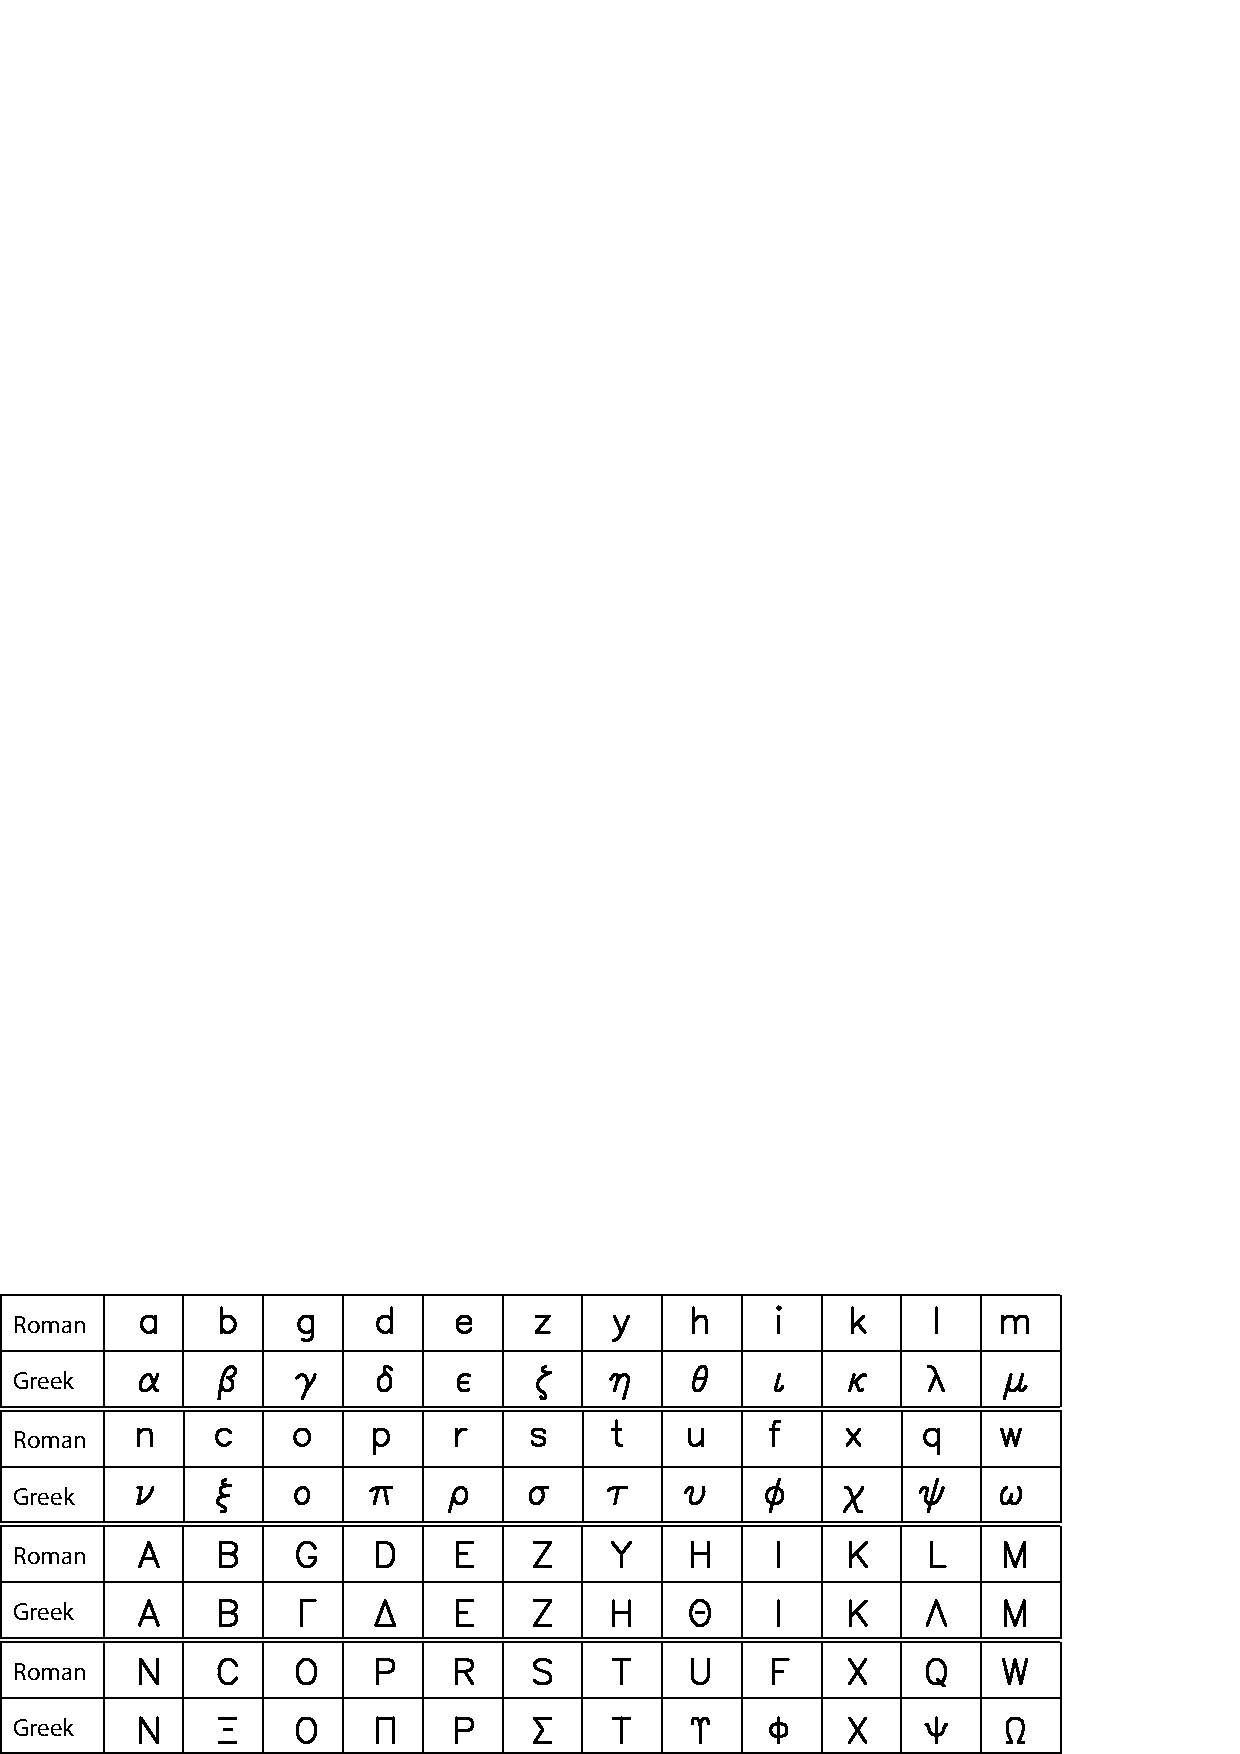
\includegraphics[width=5.0in]{greek.pdf}
  \caption[Roman to Greek Character Conversion]{Conversion for the string 
\vn{"{\B}g<r>"} where \vn{"<r>"} is a Roman character to the corresponding 
Greek character.}
\label{t:greek}
\end{table}

%-----------------------------------------------------------------
\subsection{Color Names}
\label{s:qp.color}

Possible settings for color parameters are:
\begin{example}
  White   (actually the background color)       Orange          
  Black   (actually the foreground color)       Yellow_Green    
  Red                                           Light_Green         
  Green                                         Navy_Blue       
  Blue                                          Purple          
  Cyan                                          Reddish_Purple  
  Magenta                                       Dark_Grey        
  Yellow                                        Light_Grey       
\end{example}
Color names are case insensitive.

%-----------------------------------------------------------------
\subsection{Line Pattern Names}
\label{s:qp.line.pat}

Possible settings for line patterns are:
\begin{example}
  solid      ! Solid line                 dotted     ! Dotted line             
  dashed     ! Dashed line                dash_dot3  ! Dash--dot--dot--dot line
  dash_dot   ! Dash--dot line
\end{example}
Pattern names are case insensitive.

%-----------------------------------------------------------------
\subsection{Fill Pattern Names}
\label{s:qp.fill.pat}

Possible fill pattern settings for symbols are:
\begin{example}
  solid_fill                    hatched           
  no_fill                       cross_hatched     
\end{example}
Fill pattern names are case insensitive.

